\documentclass[tikz,border=10pt]{standalone}
\usepackage{tikz}
\usetikzlibrary{shapes.geometric, arrows.meta, positioning, calc, fit, backgrounds}
\usepackage{amsmath,amssymb}
\usepackage{xcolor}

% Unified Academic Color Palette
\definecolor{cInput}{RGB}{235, 248, 255}
\definecolor{bInput}{RGB}{49, 130, 206}

\definecolor{cTrans}{RGB}{240, 249, 255}
\definecolor{bTrans}{RGB}{43, 108, 176}

\definecolor{cGCN}{RGB}{230, 255, 250}
\definecolor{bGCN}{RGB}{49, 151, 149}

\definecolor{cRecurr}{RGB}{250, 245, 255}
\definecolor{bRecurr}{RGB}{128, 90, 213}

\definecolor{cHead}{RGB}{255, 245, 245}
\definecolor{bHead}{RGB}{229, 62, 62}

\definecolor{cFusion}{RGB}{254, 252, 191}
\definecolor{bFusion}{RGB}{214, 158, 46}

\definecolor{cGray}{RGB}{247, 250, 252}
\definecolor{bGray}{RGB}{160, 174, 192}

\definecolor{tDark}{RGB}{26, 32, 44}
\definecolor{tMuted}{RGB}{74, 85, 104}

\begin{document}
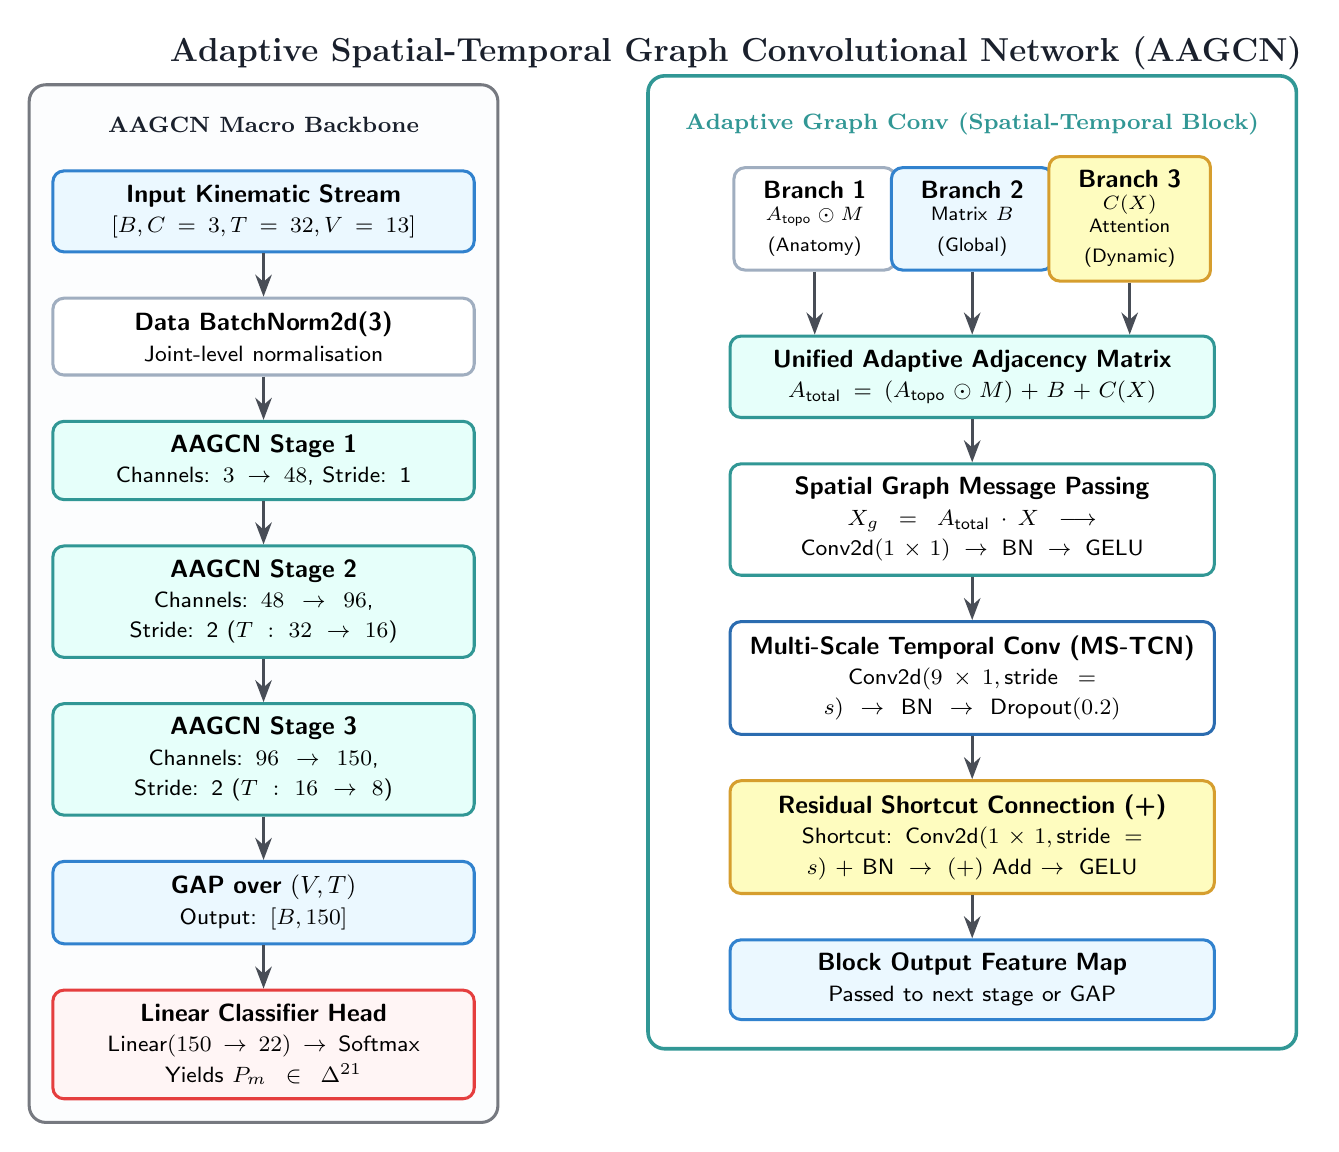
\begin{tikzpicture}[
    font=\sffamily\small,
    >=Stealth,
    node distance=0.55cm,
    block/.style={
        draw=#1,
        line width=1.1pt,
        rounded corners=4pt,
        align=center,
        inner sep=5pt
    },
    arrow/.style={->, line width=1.1pt, color=tDark!80}
]

\node[font=\bfseries\large, text=tDark] (title) at (6.0, 1.5) {Adaptive Spatial-Temporal Graph Convolutional Network (AAGCN)};

% Sub-headers
\node[font=\bfseries\footnotesize, text=tDark] (sub1) at (0, 0.6) {AAGCN Macro Backbone};
\node[font=\bfseries\footnotesize, text=bGCN] (sub2) at (9.0, 0.6) {Adaptive Graph Conv (Spatial-Temporal Block)};

% Left Column: Macro Backbone
\node[block=bInput, fill=cInput, text width=5.0cm, below=0.35cm of sub1] (m_input) {
    \textbf{Input Kinematic Stream}\\
    {\footnotesize $[B, C=3, T=32, V=13]$}
};

\node[block=bGray, fill=white, text width=5.0cm, below=of m_input] (m_bn) {
    \textbf{Data BatchNorm2d(3)}\\
    {\footnotesize Joint-level normalisation}
};

\node[block=bGCN, fill=cGCN, text width=5.0cm, below=of m_bn] (m_s1) {
    \textbf{AAGCN Stage 1}\\
    {\footnotesize Channels: $3 \to 48$, Stride: 1}
};

\node[block=bGCN, fill=cGCN, text width=5.0cm, below=of m_s1] (m_s2) {
    \textbf{AAGCN Stage 2}\\
    {\footnotesize Channels: $48 \to 96$, Stride: 2 ($T: 32 \to 16$)}
};

\node[block=bGCN, fill=cGCN, text width=5.0cm, below=of m_s2] (m_s3) {
    \textbf{AAGCN Stage 3}\\
    {\footnotesize Channels: $96 \to 150$, Stride: 2 ($T: 16 \to 8$)}
};

\node[block=bInput, fill=cInput, text width=5.0cm, below=of m_s3] (m_gap) {
    \textbf{GAP over $(V, T)$}\\
    {\footnotesize Output: $[B, 150]$}
};

\node[block=bHead, fill=cHead, text width=5.0cm, below=of m_gap] (m_head) {
    \textbf{Linear Classifier Head}\\
    {\footnotesize $\text{Linear}(150 \to 22) \to \text{Softmax}$}\\
    {\footnotesize Yields $P_m \in \Delta^{21}$}
};

\draw[arrow] (m_input) -- (m_bn);
\draw[arrow] (m_bn) -- (m_s1);
\draw[arrow] (m_s1) -- (m_s2);
\draw[arrow] (m_s2) -- (m_s3);
\draw[arrow] (m_s3) -- (m_gap);
\draw[arrow] (m_gap) -- (m_head);

% Macro background container
\begin{scope}[on background layer]
    \node[draw=tDark!60, line width=1.1pt, rounded corners=6pt, fill=cGray!40,
          fit=(sub1)(m_input)(m_head), inner sep=8pt] (macro_cont) {};
\end{scope}

% Right Column: Zoom into Adaptive Block
\node[block=bGray, fill=white, text width=1.7cm] (b1) at (7.0, -0.6) {
    \textbf{Branch 1}\\
    {\scriptsize $A_{\text{topo}}\odot M$\\(Anatomy)}
};
\node[block=bInput, fill=cInput, text width=1.7cm] (b2) at (9.0, -0.6) {
    \textbf{Branch 2}\\
    {\scriptsize Matrix $B$\\(Global)}
};
\node[block=bFusion, fill=cFusion, text width=1.7cm] (b3) at (11.0, -0.6) {
    \textbf{Branch 3}\\
    {\scriptsize $C(X)$ Attention\\(Dynamic)}
};

\node[block=bGCN, fill=cGCN, text width=5.8cm, below=0.8cm of b2] (sumA) {
    \textbf{Unified Adaptive Adjacency Matrix}\\
    {\footnotesize $A_{\text{total}} = (A_{\text{topo}} \odot M) + B + C(X)$}
};

\node[block=bGCN, fill=white, text width=5.8cm, below=of sumA] (msg) {
    \textbf{Spatial Graph Message Passing}\\
    {\footnotesize $X_g = A_{\text{total}} \cdot X \longrightarrow \text{Conv2d}(1\times 1) \to \text{BN} \to \text{GELU}$}
};

\node[block=bTrans, fill=white, text width=5.8cm, below=of msg] (tcn_blk) {
    \textbf{Multi-Scale Temporal Conv (MS-TCN)}\\
    {\footnotesize $\text{Conv2d}(9\times 1, \text{stride}=s) \to \text{BN} \to \text{Dropout}(0.2)$}
};

\node[block=bFusion, fill=cFusion, text width=5.8cm, below=of tcn_blk] (res) {
    \textbf{Residual Shortcut Connection (+)}\\
    {\footnotesize Shortcut: $\text{Conv2d}(1\times 1, \text{stride}=s) + \text{BN} \to (+)$ Add $\to \text{GELU}$}
};

\node[block=bInput, fill=cInput, text width=5.8cm, below=of res] (blk_out) {
    \textbf{Block Output Feature Map}\\
    {\footnotesize Passed to next stage or GAP}
};

\draw[arrow] (b1.south) -- (sumA.north -| b1.south);
\draw[arrow] (b2.south) -- (sumA.north);
\draw[arrow] (b3.south) -- (sumA.north -| b3.south);
\draw[arrow] (sumA) -- (msg);
\draw[arrow] (msg) -- (tcn_blk);
\draw[arrow] (tcn_blk) -- (res);
\draw[arrow] (res) -- (blk_out);

% Block background container
\begin{scope}[on background layer]
    \node[draw=bGCN, line width=1.3pt, rounded corners=6pt, fill=white,
          fit=(sub2)(b1)(b3)(blk_out), inner sep=10pt] (block_cont) {};
\end{scope}

\end{tikzpicture}
\end{document}
